\documentclass{article}
\usepackage[utf8]{inputenc}
\usepackage[a4paper, margin=2.5cm]{geometry}
\usepackage{graphicx}
\usepackage[french]{babel}

\usepackage[default,scale=0.95]{opensans}
\usepackage[T1]{fontenc}
\usepackage{amssymb} %math
\usepackage{amsmath}
\usepackage{amsthm}
\usepackage{bbm}
\usepackage{systeme}

\usepackage{hyperref}
\hypersetup{
	colorlinks=true,
	linkcolor=blue,
	filecolor=magenta,      
	urlcolor=cyan,
	pdftitle={Overleaf Example},
	pdfpagemode=FullScreen,
	}
\urlstyle{same} %\href{url}{Text}

\theoremstyle{plain}% default
\newtheorem{thm}{Théorème}[section]
\newtheorem{lem}[thm]{Lemme}
\newtheorem{prop}[thm]{Proposition}
\newtheorem*{cor}{Corollaire}
%\newtheorem*{KL}{Klein’s Lemma}

\theoremstyle{definition}
\newtheorem{defn}{Définition}[section]
\newtheorem{exmp}{Exemple}[section]
% \newtheorem{xca}[exmp]{Exercise}

\theoremstyle{remark}
\newtheorem*{rem}{Remarque}
\newtheorem*{note}{Note}
%\newtheorem{case}{Case}



\title{Simulation : Chapitre 2 : Méthode du rejet}
\author{Charles Vin}
\date{2021}

\begin{document}
\maketitle

\section{Simulation de v.a à densité}
\begin{exmp}[]
	$ f: x \mapsto \frac{1- \left| 1- \left| x \right|  \right| }{2} \mathbbm{1}_{\left| x \right| < 2}() $ est une densité de probabilité sur R. \\
	Comment faire un tirage selon la loi de densité f ? \\
	Si $ X $ suit la loi de densité $ f $  les tirages de $ X $ tombent plus fréquement là où $ f $ est élevée. 
	\[
		P(X \in  ]a-\epsilon , a]) = \int_{a_\epsilon }^{a}f(x)dx
	.\]
	Si on tire un moint au hasard dans $ \mathcal{D} $ (surface sous la courbe) on obtient un point $ (V,U) \sim Unif(\mathcal{D}) $ 
	\begin{align*}
		P(V \leq t) &= P((V,U) \text{ est dans la partie gauche du graphique } ) \\ 
			&= P((V,U) \in R, x \leq t \text{ et } 0 \leq y \leq f(x)) \\
			&= \frac{\int_{_ \infty }^{t} f(x)dx}{\int_{R}^{} f(x) dx} = \int_{-\infty }^{t}f(x) dx
	\end{align*}
\end{exmp}
\begin{exmp}[]
	Pour faire un tirage uniforme sur $ D $, on peut faire des tirage uniformes sur un $ A $ contenant $ D $ jusqu'à la première fois où le tirage tombe dans $ D $   
\end{exmp}

\subsection{Méthode de simulation}
\begin{itemize}
	\item On veut simuler une v.a. de densité $ f $ , pour $ f $  une fonction positive d'intégrale 1.
	\item On trouve une v.a. $ V $ qu'on sait simuler et dont la densité $ f_V $ majore $ f $ à constante près : 
	\[
		\forall x \in R, f(x) \leq f_V(x) \text{ avec une constante connue :} c \in R_+
	.\]
	\begin{rem}[]
		$ \int_{R}^{}f(x)d \lambda (x) = 1 \leq c \int_{R}^{}f_V(x)d \lambda (x) = c*1$ donc $ c \geq 1$  
	\end{rem}
	\begin{note}[]
		On majore une densité pas pratique pour les tirages pas une densité plus pratique dont on sait faire les tirages
	\end{note}

	\item On fait des tirages successifs de $(V_1, U_1), (V_2, U_2), \dots$ avec les $ V_i $ i.i.d. de même loi que $ V $ et les $ U_i $ i.i.d. de loi $ Unif(]0;1[) $, les $ U_i $ indépendants des $ V_i $ 
	
	\item Le premier indice $ i $ tel que 
	\[
		cf_v(V_i)U_i \leq f(V_i)
	.\]
	donne un $ X=V_i $ de densité $ f $.
	\begin{note}[]
		J'ai une valeur tiré au hasard $V_1$, je calcul mes deux densité $f_b$ et $f$, je multiplie par la constante et par un nombre tiré au hasard 0 et 1, et je regarde si l'inégalité à lieu.
	\end{note}
\end{itemize}
\begin{thm}[]
	\begin{figure}[!htbp]
		\centering
		\includegraphics*[width=\textwidth]{figures2/fig1.png}
		\caption{Exemple de tirage valide ou non}
		\label{fig1}
	\end{figure}      
	Si $(T=\inf \{i \in \mathbb{N}, cf_V(V_i)U_i \leq f(V_i)\})$ (le i correspondant au premier tirage qui satisfait l'inégalité) alors $ V_T $ suit la loi de densité $ f $. Voir figure \ref{fig1}
\end{thm}
\subsection{Pourquoi ça marche (preuve)}
On sait que $ P((V_1,U_1) \in \mathcal{D}) = \iint_{R^2}^{} \mathbbm{1}_{(v,u)\in D}f_V(v) \mathbbm{1}_{]0;1[}(u) d \lambda (v) d \lambda (u))$ car $ V_1 $ et $ U_1 $ sont indépendantes. \\
Pour $ D={(v,u) \in R^2, cf_V(v)u \leq f(V_1) \text{ et } V_1 \leq t} $ avec $ t \in R $ fixée 
\begin{align*}
	P(cf_V(v)u \leq f(V_1) \text{ et } V_1 \leq t) &= \int_{R}^{} \int_{R}^{} \mathbbm{1}_{cf_V(v)u \leq f(V_1) \text{ et } V_1 \leq t} f_V(v) \mathbbm{1}_{]0;1[}(u)d \lambda (u) d \lambda (v) \\
		&= \int_{R}^{} \int_{R}^{} \mathbbm{1}_{cf_V(v)u \leq f(V_1)} \mathbbm{1}_{ V_1 \leq t} f_V(v) \\
		&= \int_{R}^{}\mathbbm{1}_{v \leq t}f_V(v) (\int_{0}^{1}\mathbbm{1}_{cf_V(v)u \leq f(v)}d \lambda (u))
\end{align*}
Or ce qu'il y a dans la parenthèse vaut : 
\[
	\int_{0}^{1}\mathbbm{1}_{cf_V(v)u \leq f(v)}d \lambda (u) = \systeme*{
		\int_{0}^{f(v)/cf(v)} d \lambda (u) = \frac{f(v)}{cf_V(v)} \text{ si } f(v) \neq 0, 
		\int_{0}^{1}1 d \lambda (u) = 1 \text{ si } f_V(v)=0
	} = \frac{f(v)}{c} \text{ car si } f_V(v) = 0 \text{ alors } f(v) = 0, 0 \leq f \leq cf_V
.\]
\begin{align*}
	P(cf_V(v)u \leq f(V_1) \text{ et } V_1 \leq t) &= \int_{R}^{}\mathbbm{1}_{v \leq t}\frac{f(v)}{c} d \lambda (v) \\
	&= \frac{1}{c} \int_{-\infty }^{t}f(v) d \lambda (v)
\end{align*}
De même $ P(cf_V(V_1) U_1 \leq f(V_1)) = \frac{1}{c}$. Ceci étant vrai pour chaque étape $ (V_i, U_i) $, je peux calculer 
\begin{align*}
	P(V_T \leq t) &= \sum_{n=1}^{+\infty } P(V_T \leq \text{ et } T=n) \\
				&= \sum_{n=1}^{+\infty }P(\bigcap_{i=1}^{n-1}\{cf_V(V_i)U_i > f(V_i)\} \cap \{cf_V(V_n) U_n \leq f(V_n) \text{ et }V_n \leq t\}) \\
				&= \sum_{n=1}^{+\infty } (1- \frac{1}{c})^{n-1} \frac{1}{c} \int_{-\infty }^{t} f(v) d \lambda (v) \\
				&= 1 * \int_{-\infty }^{t} f(v) d \lambda (v) 
\end{align*}
donc $ V_T $ a pour densité $ f $ 

\subsection{Efficacité de la méthode}
Le nombre $ T $ de tirage de $ (V_i,U_i) $ jusqu'au premier $ V_i $ acceptable suit la loi $ Geom(\frac{1}{c}) $. 

Il faut donc en moyenne $ E(T) = c $ tirages de $(V_i,U_i)$ pour obtenir un tirage selon la densité $ f $. 

Il faut donc prendre $ c $ le plus petit possible pour rendre la méthode du rejet efficace.

\begin{exmp}[]
	Simuler la loi de densité $ f: \mapsto \frac{1-\left| \left| x \right| -1 \right| }{2} \mathbbm{1}_{\left| x \right| \leq 2}$. Voir figure \ref{fig2} \\
	\begin{figure}[!htbp]
		\centering
		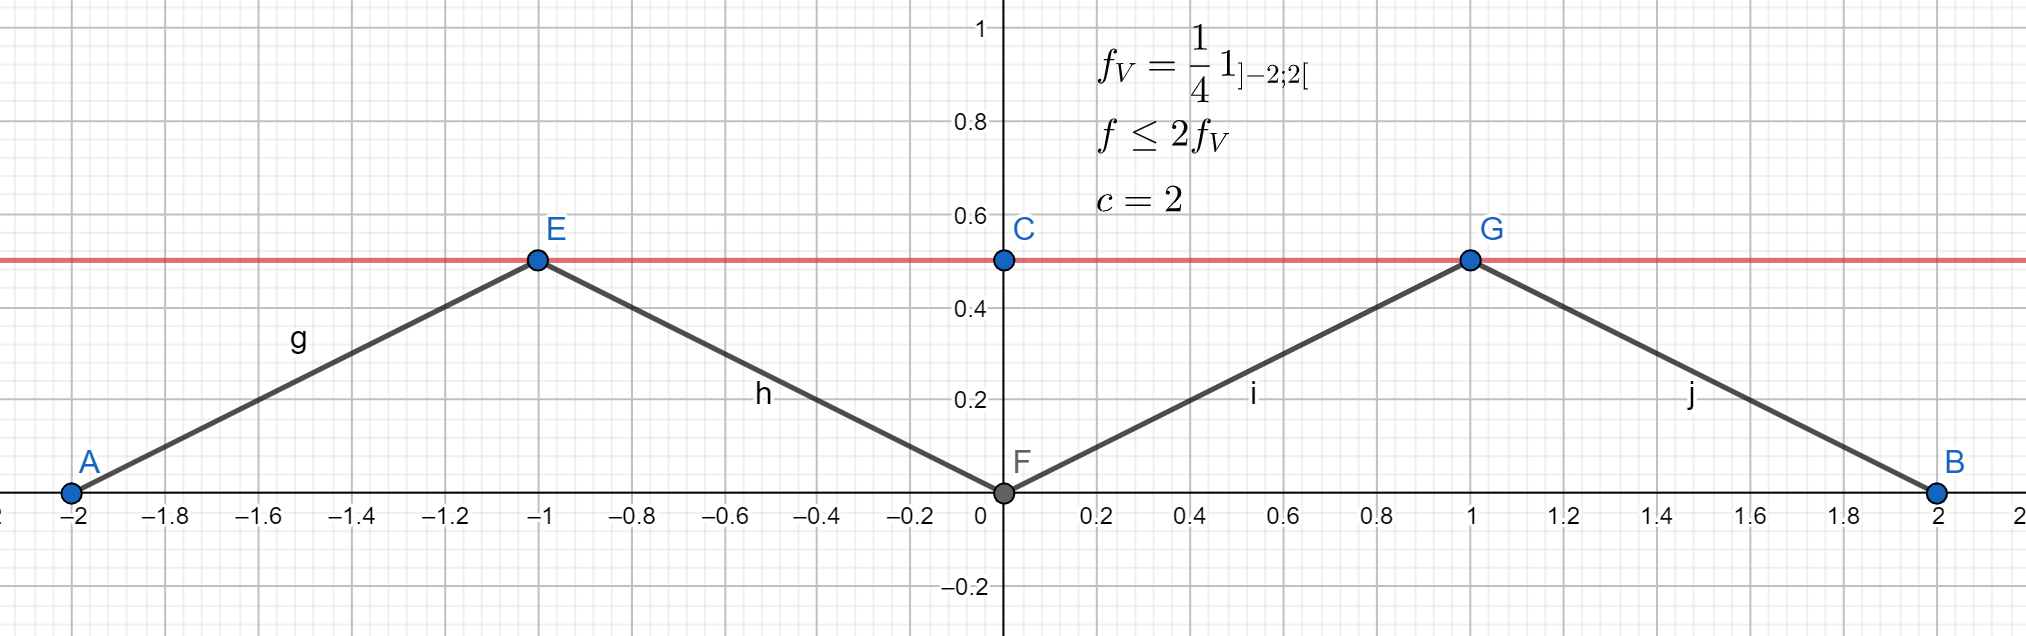
\includegraphics[width=0.85\textwidth]{figures2/fig2.png}
		\caption{Exemple 1.3}
		\label{fig2}
	\end{figure}
	On sait simuler $ V \sim Unif(]-2;2[) $ par $ V=4W-2 $ avec $ W \sim Unif(]0,1[) $. On tire $ V_1 Unif(]-2;2[) $  et $ U_1 Unif(]-0;1[) $ indépendantes, on accepte ce $ V_1(w) $ si \begin{align*}
		&2 * \frac{1}{4}\mathbbm{1}_{]-2;2[}(V_1) \leq f(V_1) \\
		& \frac{1}{2}*1*U_1 \leq frac{1-\left| \left| V_1 \right| -1 \right| }{2} *1 \\
		& U_1 \leq 1-\left| \left| V_1 \right| -1 \right| 
	\end{align*}
	Sinon on rejette $ V_1 $ et on tire $ (V_2, U_2) $ on accepte ce $ V_2 $ si $ U_2 \leq 1 - \left| \left| V_2 \right| -1 \right|  $, sinon on recommence ... \\
	En moyenne en 2 étapes, on obtient un tirage $ V_T $ de densité $ f $. 
\end{exmp}

\section{Simulations de v.a. discrète}
On va décrire la méthode du rejet pour les loi portées par $ \mathbb{N} $ (les valeurs qu'on peut tirer sont dans $ \mathbb{N} $). \\
La méthode s'adapte facilement à toute loi portée par un ensemble fini ou dénombrable
\begin{exmp}[]
	La loi de Borel de paramètre $ \mu \in [0;1] $ est donnée par 
	\[
		\forall k \in N^*, P(X=k) = \frac{e^{\mu k}*(\mu k)^{k-1}}{k!}
	.\]
	Comment simuler la loi de Borel de paramètre $ \frac{1}{2} $ ?\\
	Question : On a une famille $ (p_k)_{k \in N} $ de réel positifs tels que $ \sum_{k=1}^{+\infty} p_k=1 $. On doit construire une v.a. $ Y $ telle que $ \forall k \in N, P(Y=k) = p_k$. \\
	Idée  L'histogramme des $ (p_k)_{k \in N} $ comporte un rectangle de hauteur $ p_k $ sur chaque intervalle $ [k-\frac{1}{2};k+\frac{1}{2}] $. Il définit une zone de surface totale 1. En tirant au hasard dans cette zone, on a pour chaque nombre $ k $ une probabilité $ p_k $ de le tirer 
	\begin{figure}[htbp]
		\centering
		\includegraphics*[width=.80\textwidth]{figures2/fig3.png}
		\caption{Exemple Borel}
		\label{fig3}
	\end{figure} 
\end{exmp}

\subsection{Méthode du rejet}
\begin{itemize}
	\item On trouve une va $ V $ qu'on sait simuler et une constance $ c $ telle que $ \forall k \in N, p_k \leq c q_k $ où $ q_k = P(V=k) $\\
	Remarque : $ c \geq 1 $ car $ \sum_{k}^{}p_k =1  \leq c \sum_{k}^{}q_k = c *1$
	
	\item On fait des tirages indépendants de $ (V_1,U_1), \dots $ avec \begin{itemize}
		\item ses $ V_i $ iid de même loi que V.
		\item Les $ U_i $ iid de loi $ Unif(]0;1[) $.
		\item Les $ V_i $ indépendants des $ U_i $.
	\end{itemize}
	
	\item On prend $ Y(w) = V_i(w) $ pour le premier indice $ i $ tel que $ c q_{V_i} U_i \leq P_{V_i}$. \\
	$ Y $ ainsi construit satisfait $ \forall k \in N, P(Y=k) = p_k $  
\end{itemize}

\underline{Nouveau cours du 19/10} \\

\begin{proof}[Preuve de la méthode : ]
	\begin{align*}
		P(V_1 = k \text{ et } cq_k U_1 \leq p_k) &= P(V_1=k) P(cq_kU_1 \leq P_k) \\
		&= q_kP(U_1 \leq \frac{p_k}{cq_k}) \\
		&= q_k \frac{p_k}{cq_k} = \frac{p_k}{c}
	\end{align*}
	Et si $ q_k = 0 $ ? Alors $ p_k=0 $ donc même résultat. 

	Probabilité d'accepter $ V_1 $ : \begin{align*}
		P(cq_{V_1}U_1 \leq p_{V_1}) &= \sum_{k=0}^{+\infty }P(V_1=k \text{ et } cq_kU_1 \leq p_k) \\
		&= \sum_{k)1}^{+\infty }\frac{p_k}{c} = \frac{1}{c}
	\end{align*}
	\begin{align*}
		P(Y=k) &= P(V_n = k \text{ pour N le premier indice i tel que } cq_{V_i}U_i \leq P_{V_i})
		&= \sum_{n=1}^{+\infty }P(cq_{V_1} \text{ et } cq_{V_2}U_2 > P_{V_2} \text{ et } \dots \text{ et } cq_{V_{n-1}}U_{n-1} > P_{V_{n-1}} \text{ et } cq_{V_{n}}U_{n} > P_{V_{n}} \text{ et } V_n=k)\\
		&= \text{ tous de proba } 1 - \frac{1}{c} \text{ indépendants} \\
		&= \sum_{n=1}^{+\infty }(1-\frac{1}{c})^{n-1} \frac{p_k}{c} \\
		&= p_k \sum_{n=1}^{+\infty }\frac{1}{c} (1-\frac{1}{c})^{n-1} \text{ (Loi géométrique (1/c))} \\
		&= p_k * 1 = P(X=k), \forall k \in \mathbb{N}
	\end{align*}
	CCL : $ Y $ simule $ X $. \\
	Le nombre d'étapes pour obtenir un tirage de $ X $ suit une loi $ \mathcal{G}eom(\frac{1}{c}) $. Il faut en moyenne $ c $ étapes pour 1 tirage
\end{proof}

\begin{exmp}[Simulation de la loi de Borel de paramètre 1/2]
	\[
		p_k = \frac{e^{-\frac{k}{2}} (\frac{k}{2})^{k-1}}{k!} = \frac{e^{-\frac{k}{2} k^{k-1}}}{k! 2^{k-1}}, \forall k \in \mathbb{N}^*
	.\]
	Pour $ q_k $ prendre une Poisson ? \begin{align*}
		p_k \leq c q_k \Leftrightarrow & \frac{e^{-\frac{k}{2} k^{k-1}}}{k! 2^{k-1}} \leq c e^{-\lambda } \frac{\lambda ^k}{k!}\\
						\Leftrightarrow & k^{k-1} \leq c e^{-\lambda }e^{\frac{k}{2} 2^{k-1}} \\
						\Leftrightarrow & \frac{k^k}{k} \leq \frac{ce^{-\lambda }}{2}(\lambda \sqrt[]{e}2)^k \\
						\Leftrightarrow & \frac{1}{c} \leq \frac{e^{-\lambda }}{2} (\frac{(\lambda \sqrt[]{e}2)^k}{k^k}k)_{ \to_{k \to +\infty} 0}
	\end{align*}
	Pour $ q_k $ prendre une géométrique ? $ \frac{q_{k+1}}{q_k} = 1 - \text{ paramètre } $ \begin{align*}
		\frac{p_{k+1}}{p_k} &= \frac{e^{- \frac{k+1}{2} (k+1)^k}}{(k+1)! 2^k} * \frac{k! 2^{k-1}}{e^{-\frac{k}{2}} k^{k-1}} \\
				&= \frac{e^{-\frac{1}{2}} k}{(k+1)2} (\frac{k+1}{k})^k \\
				&= \frac{e^{1/2}}{2} \frac{k}{k+1} (1+\frac{1}{k})^k \leq \\
				&= \frac{1}{2 \sqrt[]{e}} \frac{k}{k+1}e^{k \ln (1+\frac{1}{k})}
				& \leq \frac{1}{2 \sqrt[]{2}}e^1 \frac{\sqrt[]{e}}{2} \text{ car } \ln (1+ \frac{1}{k}) \leq \frac{1}{k}
	\end{align*} 
	\begin{align*}
		\forall k \in \mathbb{N}^*, & p_k \leq (\frac{\sqrt[]{e}}{2})^{k-1}p_1 = (\frac{\sqrt[]{e}}{2})^{k-1} \frac{1}{\sqrt[]{e}} = c q_k
									& p_k \leq (1-\frac{\sqrt[]{e}}{2})(\frac{\sqrt[]{e}}{2})^{k-1} * \frac{2}{2- \sqrt[]{e}}\frac{1}{\sqrt[]{e}} \\
									& Geom(1-\frac{\sqrt[]{e}}{2}) * c 
	\end{align*}
	On fait des tirages indépendants de $ (V_i,U_i) $ avec les $ V_i \sim Geom(1-\frac{\sqrt[]{e}}{2}) $ et $ U_i \sim Unif(]0;1[) $ independante des $ V_i $ jusqu'au premier tirage où 
	\[
		\frac{2}{(2-\sqrt[]{e})\sqrt[]{e}}(1-\frac{\sqrt[]{e}}{2})(\frac{\sqrt[]{e}}{2})^{V_i} U_i \leq \frac{e^{-V_i /2}(V_i / 2)^{V_i -1}}{V_i !}
	.\]
\end{exmp}

\section{Simulation de vecteurs aléatoires à densité}
\begin{prop}[]
	Soit $ f: \mathbb{R}^d \to \mathbb{R} $ une application positive d'intégrale 1. 

	Si $ V_1, V_2, \dots $ est une suite de vecteurs aléatoire à valeur dans $ \mathbb{R}^d $ i.i.d. de densité $ f_V $ telle que $ f \leq cf_V $ pour une constance $ c \in \mathbb{R} $. \\
	Alors $ U_1, U_2, \dots $ des v.a. i.i.d. $ \sim Unif(]0;1[) $ indépendantes des $ V_i $ on a pour $ T = \inf \{i \in \mathbb{N}^*, c f_V(V_i)U_i \leq f(V_i)\} $ 
	\begin{itemize}
		\item $ T \sim Geom(\frac{1}{c}) $ 
		\item $ V_T $ a pour densité $ f $ 
	\end{itemize}
	\begin{proof}[Preuve: ]
		Analogue à la dimension 1
	\end{proof}    
\end{prop}
\textbf{Rappel:} loi uniforme sur un pavé de $ \mathbb{R}^2 $ \\ 
Si $ U_1,U_2, \dots, U_d $ sont indépendantes de loi $ U_k \sim Unif(]a_k,b_k[) $ pour chaque $ k $, alors 
\[
	(U_1, U_2,\dots,U_d) \sim Unif(]a_1,b_1[ \times ]a_2,b_2[ \times \dots \times ]a_d, b_d[)
.\]
\begin{proof}[Preuve: ]
	\textbf{Rappel:} si $ \mathcal{D} \subset \mathbb{R}^2 \in Bor(\mathbb{R}^2), U \sim Unif(D) $ si $ \forall A \in Bor(\mathbb{R}^2), P(U \in A) = \frac{\lambda (A \cap D)}{\lambda (D)} $ 
	\begin{align*}
		P((U_1, U_2) \in A) &= \int_{\mathbb{R}^2}^{}\mathbbm{1}_{(u_1,u_2) \in A} f_{U_1}(u_1) * f_{U_2}(u_2) d \lambda (u_1) d \lambda (u_2) \\
							&= \int_{\mathbb{R}} \int_{\mathbb{R}}^{} \mathbbm{1}_{(u_1,u_2) \in A} \frac{1}{b_1 - a_1} \mathbbm{1}_{a_1 \leq u_1 \leq b_1} \frac{1}{b_2 - a_2} \mathbbm{1}_{a_2 \leq u_2 \leq b_2} d \lambda (u_1) d \lambda (u_2) \\
							&= \frac{1}{(b_1-a_1)(b_2-a_2)} \lambda (A \cap (]a_1,b_1[ \times ]a_2,b_2[)) \\
							&= \frac{1}{\lambda (]a_1,b_1[ \times ]a_2,b_2[)} \lambda (A \cap (]a_1,b_1[ \times ]a_2,b_2[)) 
	\end{align*}
\end{proof}

\begin{prop}[Transformation affine de loi uniforme]
	Soit $ U \sim Unif(D) $ où $ D $ est une partie borélienne de $ \mathbb{R}^d $.\\
	Si $ M $ est une matrice $ d \times d $ inversible et si $ a $ est un point de $ \mathbb{R}^d $, alors le vecteur aléatoire $ MU+a $ suit la loi uniforme sur l'image $ D^\prime  $ de $ D $ par la transformation affine : $ x \mapsto Mx+a $.
\end{prop}
\begin{exmp}[]
	\begin{itemize}
		\item Tirage au hasard dans le disque unité $ D = \{(x,y) \in \mathbb{R}^2, x^2+y^2 \leq 1\} $ On tire indépendamment $ (X_1, Y_1) $ de loi $ Unif(]-1;1[) $ on répète indépendamment les tirages jusqu'au premier indice où $ X_i^2 + Y_i^2 \leq 1 $ (méthode du rejet)
		\item Tirage au hasard dans l'ellipse centrée en $ (50,50) $ de grand axe $[(0,0) , (100,100)$ et de petite axe $ [(45,55),(55,45) $ (elle est très aplatie, tirer dans le carée et rejeter les mauvais point trop long, on vas donc faire une translation) 
		\[
			\epsilon = MD + (50,50)
		.\] 
		\[
			(x_1, x_2) \mapsto (\sqrt[]{5000}x_1, \sqrt[]{50}x_2) \mapsto 
		.\]
		\begin{align*}
			M = \frac{\sqrt[]{2}}{2}\sqrt[]{50} \begin{pmatrix}
				1 & -1 \\
				1 & 1
			\end{pmatrix}
			\begin{pmatrix}
				10 & 0 \\
				0 & 1
			\end{pmatrix} = 5 \begin{pmatrix}
				10 & -1 \\
				10 & 1
			\end{pmatrix}
		\end{align*}
		Si $ (X_T, Y_T) $ uniforme sur D 
		\[
			M \binom{X_T}{Y_T}  + \binom{50}{50} = \binom{50X_T - 5Y_T + 50}{50 X_T + 5Y_T + 50} \sim Unif(\epsilon )
		.\]
	\end{itemize}
\end{exmp}



\end{document}